\documentclass[12pt, titlepage]{article}

\usepackage{fullpage}
\usepackage[round]{natbib}
\usepackage{multirow}
\usepackage{booktabs}
\usepackage{tabularx}
\usepackage{graphicx}
\usepackage{float}
\usepackage{hyperref}
\hypersetup{
    colorlinks,
    citecolor=blue,
    filecolor=black,
    linkcolor=red,
    urlcolor=blue
}

%% Comments

\usepackage{color}

%\newif\ifcomments\commentstrue %displays comments
\newif\ifcomments\commentsfalse %so that comments do not display

\ifcomments
\newcommand{\authornote}[3]{\textcolor{#1}{[#3 ---#2]}}
\newcommand{\todo}[1]{\textcolor{red}{[TODO: #1]}}
\else
\newcommand{\authornote}[3]{}
\newcommand{\todo}[1]{}
\fi

\newcommand{\wss}[1]{\authornote{blue}{SS}{#1}} 
\newcommand{\plt}[1]{\authornote{magenta}{TPLT}{#1}} %For explanation of the template
\newcommand{\an}[1]{\authornote{cyan}{Author}{#1}}

%% Common Parts

\newcommand{\progname}{Mechatronics Engineering} % PUT YOUR PROGRAM NAME HERE
\newcommand{\authname}{Team 25, Preliminary
\\ Ahmed Nazir, nazira1
\\ Stephen Oh, ohs9
\\ Muhanad Sada, sadam
\\ Tioluwalayomi Babayeju, babayejt} % AUTHOR NAMES                  

\usepackage{hyperref}
    \hypersetup{colorlinks=true, linkcolor=blue, citecolor=blue, filecolor=blue,
                urlcolor=blue, unicode=false}
    \urlstyle{same}
                                


\newcounter{acnum}
\newcommand{\actheacnum}{AC\theacnum}
\newcommand{\acref}[1]{AC\ref{#1}}

\newcounter{ucnum}
\newcommand{\uctheucnum}{UC\theucnum}
\newcommand{\uref}[1]{UC\ref{#1}}

\newcounter{mnum}
\newcommand{\mthemnum}{M\themnum}
\newcommand{\mref}[1]{M\ref{#1}}

\begin{document}

\title{System Design for \progname{}} 
\author{\authname}
\date{\today}

\maketitle

\pagenumbering{roman}

\section{Revision History}

\begin{tabularx}{\textwidth}{p{3cm}p{2cm}X}
\toprule {\bf Date} & {\bf Version} & {\bf Notes}\\
\midrule
Date 1 & 1.0 & Notes\\
Date 2 & 1.1 & Notes\\
\bottomrule
\end{tabularx}

\newpage

\section{Reference Material}

This section records information for easy reference.

\subsection{Abbreviations and Acronyms}

\renewcommand{\arraystretch}{1.2}
\begin{tabular}{l l} 
  \toprule		
  \textbf{symbol} & \textbf{description}\\
  \midrule 
  \progname & Explanation of program name\\
  \wss{...} & \wss{...}\\
  \bottomrule
\end{tabular}\\

\newpage

\tableofcontents

\newpage

\listoftables

\listoffigures

\newpage

\pagenumbering{arabic}

\section{Introduction}

The system design document establishes the group's development considerations for the Formulate system. The motivations which drove each aspect of the design were referenced back to the System Requirements Specification, Hazard Analysis, and Development Plan documents. 

\wss{Include references to your other documentation}

\section{Purpose}

\wss{Purpose of your design documentation}

\wss{Point to your other design documents}

Documentation of the Formulate system's design serves to improve the maintainability, reusability, and understandability of the project. This is accomplished through the system design, software architecture, and software detailed design documents by detailing how the design addressed the requirements outlined in the documents from this document's introduction. \\

\section{Scope}

\wss{Include a figure that show the System Context (showing the boundary between
your system and the environment around it.)}

This document in particular focuses on the considerations for the user interface, mechanical, electrical, and communication protocol aspects of the system. All relevant design decisions relating to the requirements were detailed by each aspect of the system, and any visual components used to aid the design were included at the end of the document by each aspect of the system. \\ 

\subsection{System Context Diagram}
\begin{figure}[h!]
  \begin{center}
  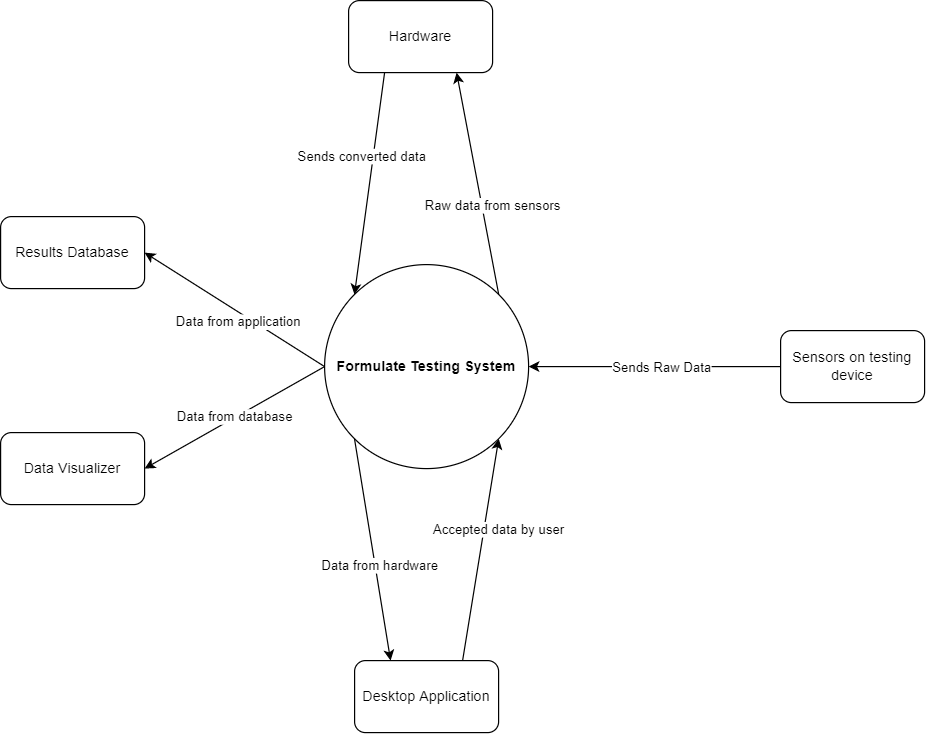
\includegraphics[width=1.1\textwidth]{sys_context_diagram}
  \caption{Formulate Context Diagram}
  \end{center}
  \end{figure}
  \newpage

\section{Project Overview}

\subsection{Normal Behaviour}

\subsection{Undesired Event Handling}

\wss{How you will approach undesired events}

\subsection{Component Diagram}

\subsection{Connection Between Requirements and Design} \label{SecConnection}

\wss{The intention of this section is to document decisions that are made
  ``between'' the requirements and the design.  To satisfy some requirements,
  design decisions need to be made.  Rather than make these decisions implicit,
  they are explicitly recorded here.  For instance, if a program has security
  requirements, a specific design decision may be made to satisfy those
  requirements with a password.}

\section{System Variables}

\wss{Include this section for Mechatronics projects}

\subsection{Monitored Variables}

\subsection{Controlled Variables}

\subsection{Constants Variables}

\section{User Interfaces}

\wss{Design of user interface for software and hardware.  Attach an appendix if
needed. Drawings, Sketches, Figma}

\section{Design of Hardware}

\wss{Most relevant for mechatronics projects}
\wss{Show what will be acquired}
\wss{Show what will be built, with detail on fabrication and materials}
\wss{Include appendices as appropriate, possibly with sketches, drawings, CAD, etc}

\newpage
\section{Design of Electrical Components}

\wss{Most relevant for mechatronics projects}
\wss{Show what will be acquired}
\wss{Show what will be built, with detail on fabrication and materials}
\wss{Include appendices as appropriate, possibly with sketches, drawings,
circuit diagrams, etc}

The electrical components were selected to address the functional requirements regarding robust sensor connection points, wireless functionality, and backup data collection capabilities. These capabilities were enabled using hardware modules selected to interface with the embedded device. \\

The Arduino Uno R3 (Uno) was the choice electrical component for the devices embedded hardware. While other embedded devices  were also capable of flexibly collecting data from a multitude of sensors, the Uno stood out as the optimal choice because of low monetary cost in hardware and the relatively high accessibility at large e-commerce platforms for the Formula Electric Team to purchase. In addition, the likelihood of the Formula Electric team using parts of the testing budget on the embedded hardware was minimized as many Formula Electric members already posessed an Uno board. \\

To support testing application flexibility in cases where no direct connections to power were available, four 1.5 volt batteries with a battery holder was used to provide the Uno with adequate power for on vehicle testing sessions. \\

A single pole, double throw (SPDT) power switch was used to easily connect and disconnect the four 1.5 volt batteries with the circuit connecting all electrical components. This gave the user to The common pin actuated to connect either the 9V battery to the circuit or the circuit directly to ground. \\

Although the Uno provided many functionalities, the standard Uno model did not natively support wireless communication capabilities. As a result, the group chose to integrate a hardware module capable of a Transmission Control Protocol / Internet Protocol (TCP/IP) stack through an ESP8266 Software On Chip (SOC). The electrical component containing the ESP8266 SOC that was selected was the Node MCU 1.0. The Node MCU 1.0 is a development board with the ESP8266 SOC already built onto the Node MCU's PCB in addition to an on-board voltage regulator for the development boards 3.3 volt power in requirement. \\

A single pole, single throw (SPST) switch packaged with four ports was also required to interface the Node MCU 1.0 module with the Uno during initial device comissioning. Specifically, three of the four ports were used to disconnect the 3.3 volt power, transmit (TX), and recieve (RX) signal between the wifi module and the embedded device when flashing the wifi module with firmware via a micro Universal Serial Bus (USB) port. When the one time firmware flash is complete, the three switches could be actuated to reconnect the power and signal connections between the two components. Despite the connect/disconnect functionality requiring only three of the four ports, a four port SPST switch was selected due to the high accesibility on large electronics e-commerce platforms relative to three port SPST switches. \\

Two diagnostic light-emitting diode's (LED) were used to provide the user with feedback on the live transmission status of the wifi module. The first diagnostic signal conveyed when a connection between the wifi module and the desktop application was established, showing the module was capable of transmitting data. This required the first LED to visually depict the active signal to the user. The second diagnostic signal conveyed when the wifi module was actively transmitting data live to the desktop application. This required the second LED to visually depict the active signal to the user. \\

Two resistors were also paired with the diagnostic LED's to primarily limit the current going through each LED, but also the luminosity of both LED's. Limiting the current through each LED was an important consideration as it supports a consistent luminoscity in the LED's and mitigates premature breakdown of the LED due to a high current burnout. \\

Backup data storage to local memory in the event of wireless communication error due to the wifi module's failure or device operation outside the wifi router's range necessitated the use of a local memory storage electrical component. A 32 GigaByte (GB) micro Secure Digital (SD) card paired with a micro SD card adapter was used to provide the Uno with local memory storage to concurrently write test data to the SD card while also sending data over wifi to the desktop application. SanDisk, the microSD card manufacturer, was chosen primarily due to their cost effectiveness against other microSD manufacturers as measured by GB/dollar. Similarly, Geek Story was used as the microSD card adapter manufacturer as a result of their cost-effectiveness. \\

Robust sensor connection components between the sensor and the Uno's input ports were required for tests in physically demanding scenario's as loose or broken connections from high vibration or shock compromised the reliability of the sensor readings and thus the test data. As a result, Phoenix Contact's through hole, 8 port terminal blocks were used because the terminal block style connections provided a stronger connective interface between the sensor conductors and the Uno's ports. \\

Robust connections between all components of the circuit such as the electrical connections between the Uno, wifi module, micro SD card adapter, switches, and LED's also required a more robust solution relative to jumper wires. As a result, the group chose to design and manufacture a Printed Circuit Board (PCB) onto which all electrical components outlined could be soldered onto the board for a higher strength connection. \\
\newpage

The required electrical connections between the micro SD adapters pinouts and the Uno's pinouts were first outlined to organize the connection layout in the table below. \\

\begin{table}[H]
  \centering
  \begin{tabular}{|p{2cm}|p{6cm}|p{2cm}|p{2cm}|}
  \hline
  \multicolumn{1}{|c|}{\textbf{Pin Name}} & \multicolumn{1}{c|}{\textbf{Pin Description}} & \multicolumn{1}{|c|}{\textbf{Arduino Port}} & \multicolumn{1}{|c|}{\textbf{Arduino Port Description}} 
  \\ \hline
  VCC
  & 5 Volt
  & 5 Volt
  & Power output
  \newline                                
  \\ \hline

  GND                              
  & Ground
  & Ground
  & Ground
  \newline                                
  \\ \hline

  MISO                          
  & SPI output from microSD
  & 12
  & Digital I/O
  \newline                                
  \\ \hline

  MOSI                                
  & SPI input to microSD
  & 11 
  & Digital I/O
  \newline                            
  \\ \hline

  SCK                                
  & Synchronize data transmission via Arduino clock
  & 13 
  & Digital I/O
  \newline                            
  \\ \hline

  CS                                
  & Select slave device on SPI bus
  & 10 
  & Digital I/O
  \newline                            
  \\ \hline

  \end{tabular}
\end{table}


The required electrical connections between the wifi module's pinouts and the Uno's pinouts were also outlined to organize the connection layout in the table below. \\

\begin{table}[H]
  \centering
  \begin{tabular}{|p{2cm}|p{6cm}|p{2cm}|p{2cm}|}
  \hline
  \multicolumn{1}{|c|}{\textbf{Pin Name}} & \multicolumn{1}{c|}{\textbf{Pin Description}} & \multicolumn{1}{|c|}{\textbf{Arduino Port}} & \multicolumn{1}{|c|}{\textbf{Arduino Port Description}} 
  \\ \hline
  3V3
  & 3.3 Volt
  & 3.3 Volt
  & Power output
  \newline                                
  \\ \hline

  GND                              
  & Ground
  & Ground
  & Ground
  \newline                                
  \\ \hline

  TX                          
  & Transmit
  & 2
  & Digital I/O
  \newline                                
  \\ \hline

  RX                                
  & Recieve
  & 3
  & Digital I/O
  \newline                            
  \\ \hline


  \end{tabular}
\end{table}


\newpage

A final list of the required electrical components was shown below. \\

\begin{table}[H]
  \centering
  \begin{tabular}{|p{3cm}|p{2cm}|p{4cm}|p{4cm}|p{2cm}|}
  \hline
  \multicolumn{1}{|c|}{\textbf{Component}} & \multicolumn{1}{c|}{\textbf{Manufacturer}} & \multicolumn{1}{c|}{\textbf{Part Number}} & \multicolumn{1}{c|}{\textbf{Description}} & \multicolumn{1}{|c|}{\textbf{Quantity}}
  \\ \hline
  Microcontroller
  & Arduino
  & Uno R3
  & System micro-controller
  & 1
  \newline                                
  \\ \hline

  Wifi Module                              
  & NodeMCU
  & 1.0
  & System wifi 
  & 1
  \newline                                
  \\ \hline

  Micro SD Adapter                          
  & Geek Story
  & N/A
  & Local memory interface
  & 1
  \newline                                
  \\ \hline

  Micro SD Card                                
  & Sandisk
  & SDSQUAR-032G-GN6MA
  & System local memory
  & 1
  \newline                            
  \\ \hline

  Battery                                
  & Duracell
  & 4330206640
  & System power
  & 4
  \newline                            
  \\ \hline

  SPDT Switch                                
  & E-Switch
  & 100SPTITI1B4M2QE
  & System power switch
  & 1
  \newline                            
  \\ \hline

  4 Port SPST Switch                                
  & TE
  & 435640-2
  & Wifi signal control switch
  & 1
  \newline                            
  \\ \hline

  Through Hole Terminal Block                                
  & Phoenix Contact
  & 1715789
  & System Sensor ports
  & 2
  \newline                            
  \\ \hline

  LED                                
  & Kingbright
  & WP7113ID5V
  & LED Resistor
  & 2
  \newline                            
  \\ \hline

  Resistor                                
  & TE
  & CBT25J100R
  & LED Resistor
  & 2
  \newline                            
  \\ \hline

  Custom PCB                                
  & JLCPCB
  & N/A
  & System PCB
  & 1
  \newline                            
  \\ \hline

  \end{tabular}
\end{table}

The electrical schematic for the overall circuit containing all components was designed in Kicad and was shown in Appendix C. The PCB layout was also designed in Kicad and was shown in Appendix C. The PCB layout was then fabricated by the manufacturer JLCPCB. \\

\newpage




\section{Design of Communication Protocols}

\wss{If appropriate}

\section{Timeline}

\wss{Schedule of tasks and who is responsible}

% \bibliographystyle {plainnat}
% \bibliography{../../../refs/References}

\newpage{}

\appendix

\section{Interface}

\wss{Include additional information related to the appearance of, and
interaction with, the user interface}

\section{Mechanical Hardware}


\newpage
\section{Electrical Components}

\subsection{Electrical Schematic}
\begin{figure}[h!]
  \begin{center}
  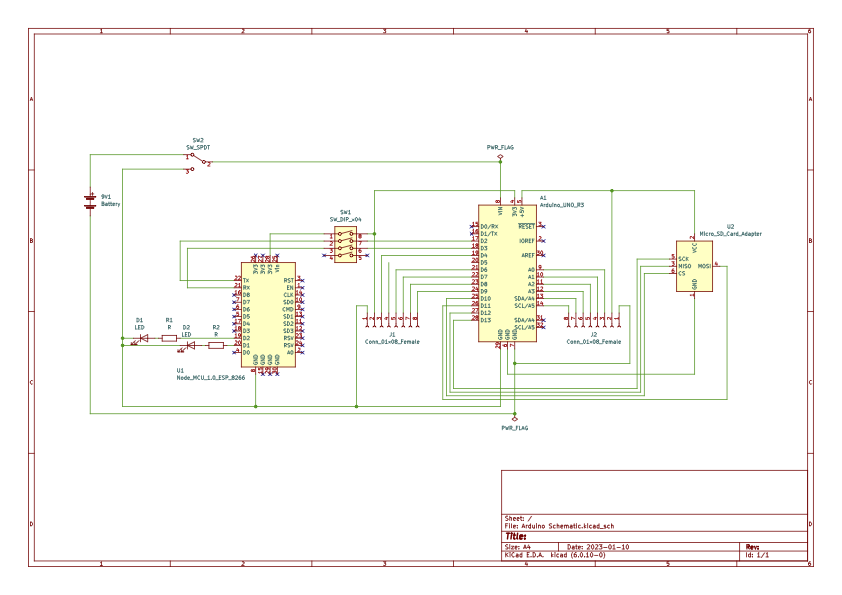
\includegraphics[width=1.1\textwidth]{Electrical_Schematic}
  \caption{Electrical Schematic in Kicad}
  \end{center}
  \end{figure}
  \newpage

\subsection{PCB Layout}
\begin{figure}[h!]
  \begin{center}
  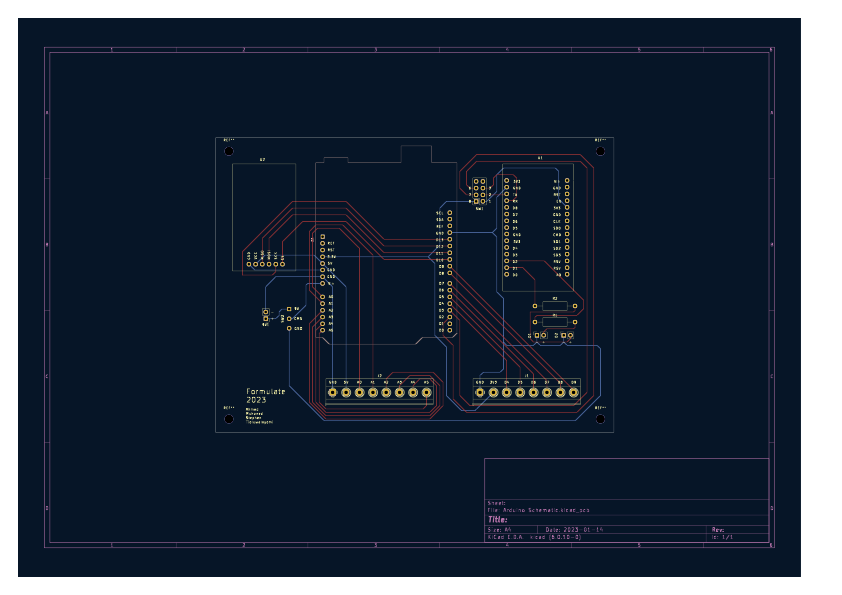
\includegraphics[width=1.1\textwidth]{PCB_Schematic}
  \caption{PCB Layout in Kicad}
  \end{center}
  \end{figure}
  \newpage

\subsection{PCB CAD}
\begin{figure}[h!]
  \begin{center}
  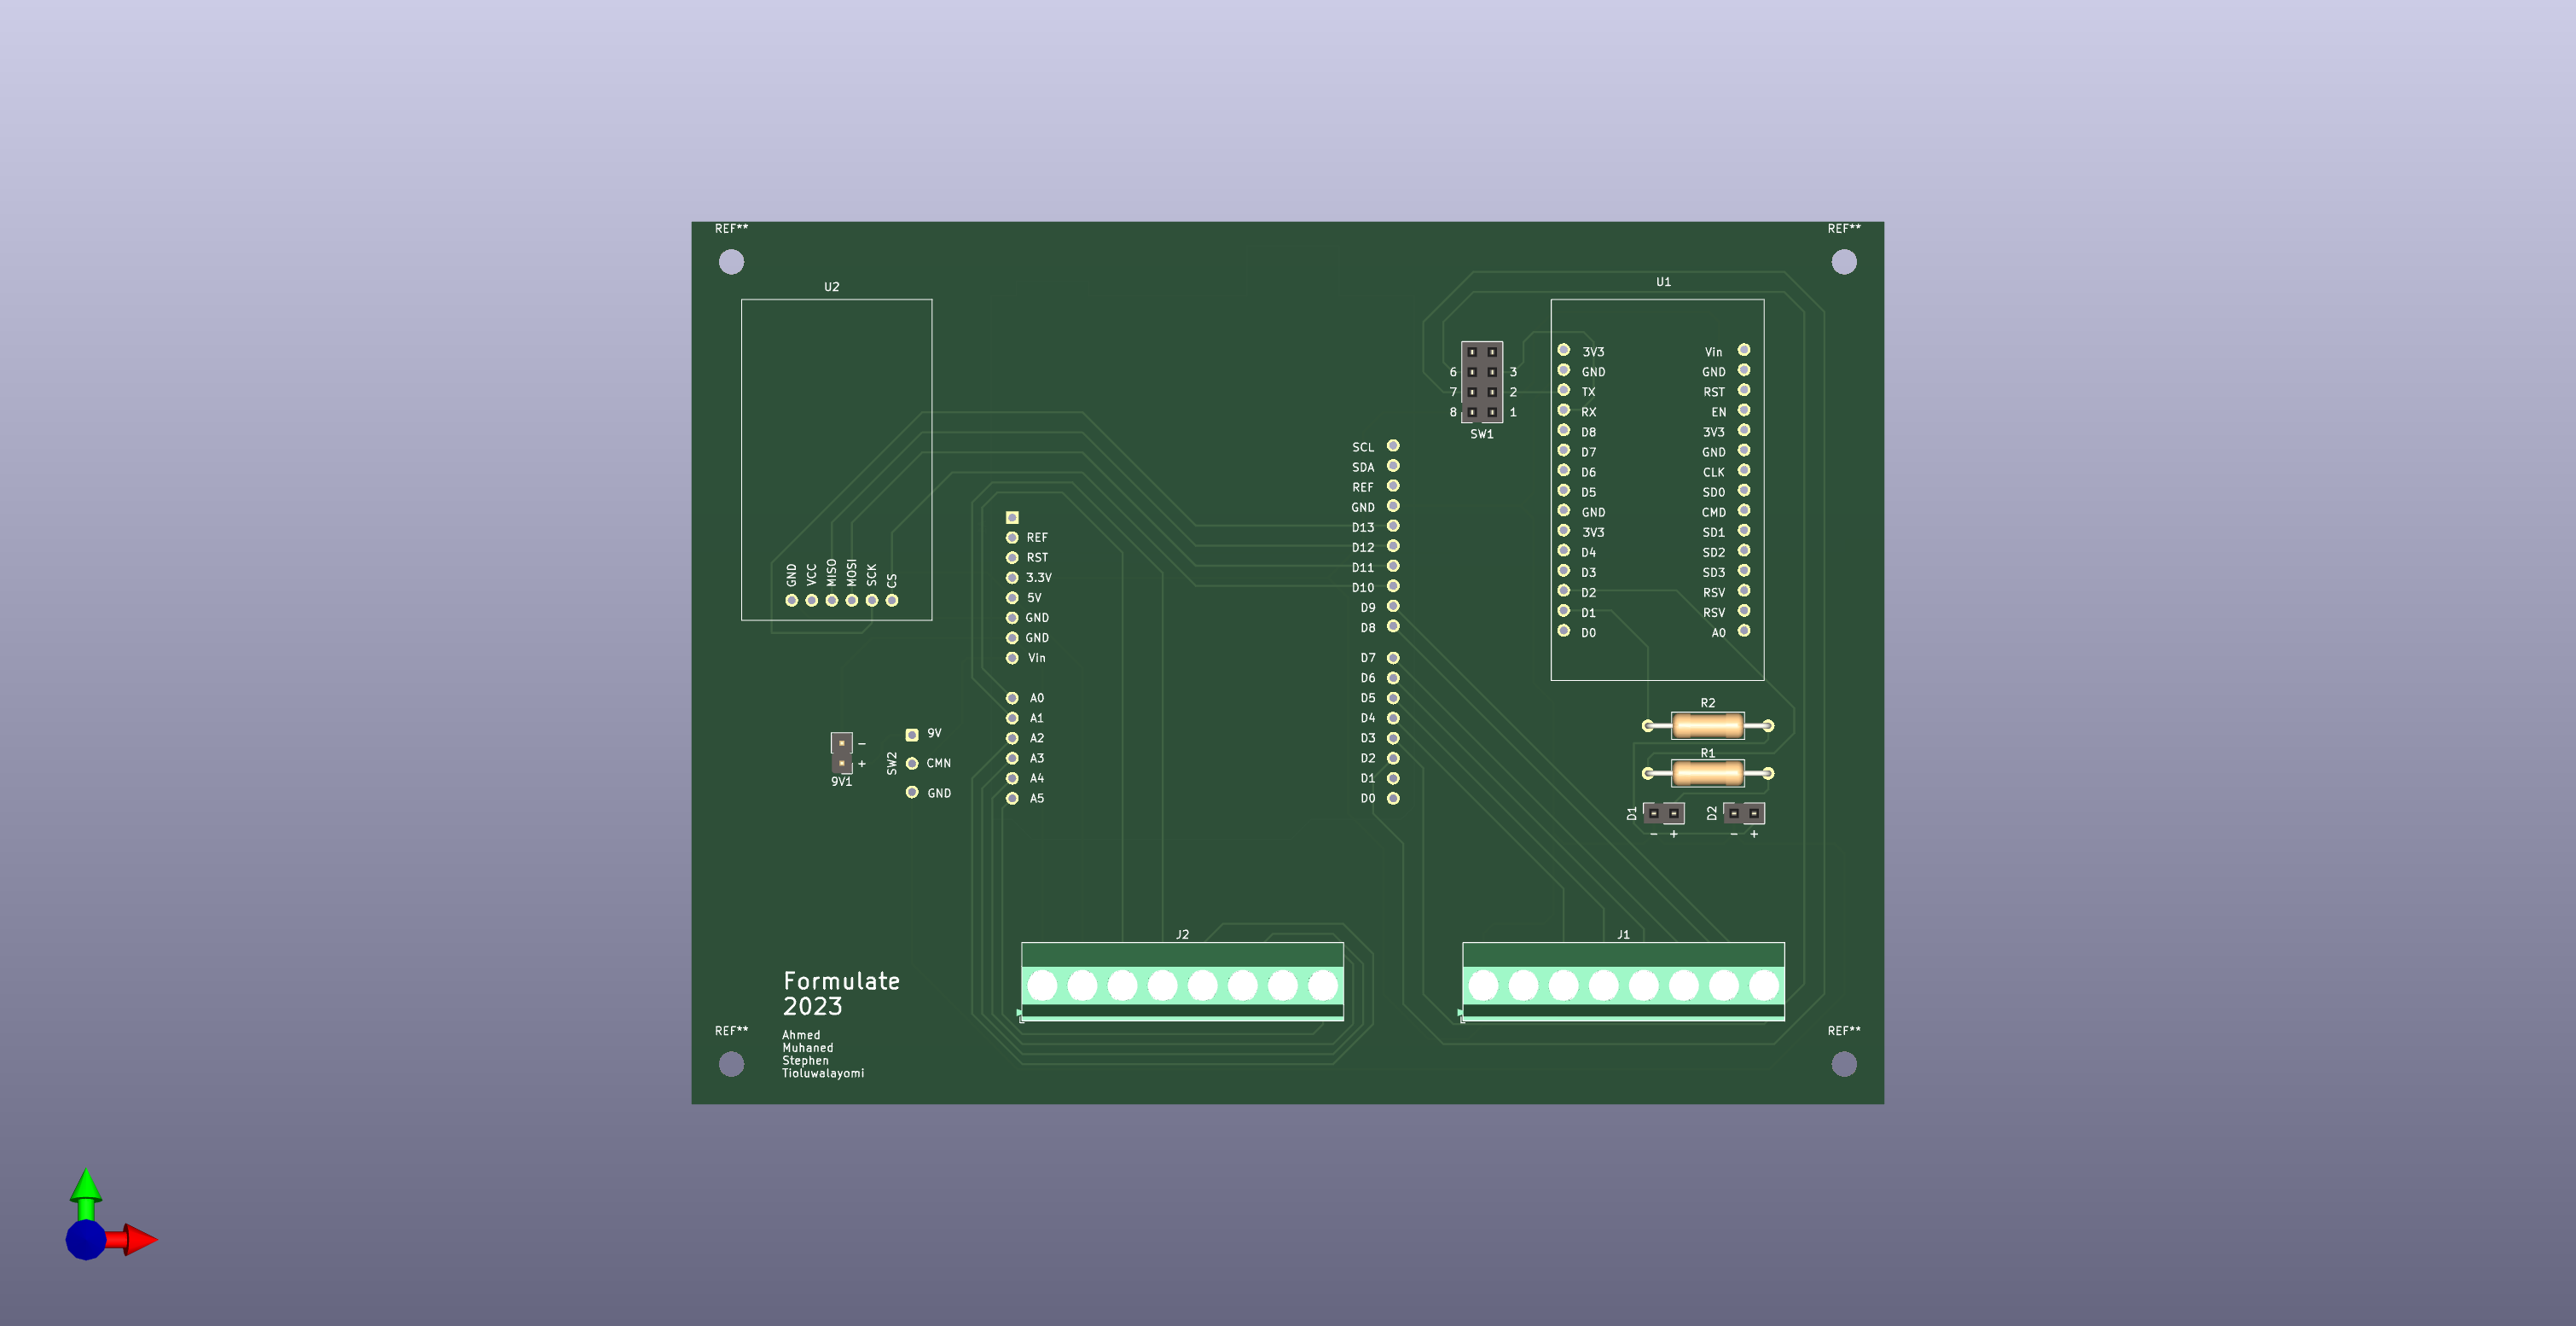
\includegraphics[width=1.1\textwidth]{PCB_Front_View}
  \caption{Top view of the PCB}
  \end{center}
  \end{figure}
  \newpage

\subsection{PCB CAD}
\begin{figure}[h!]
  \begin{center}
  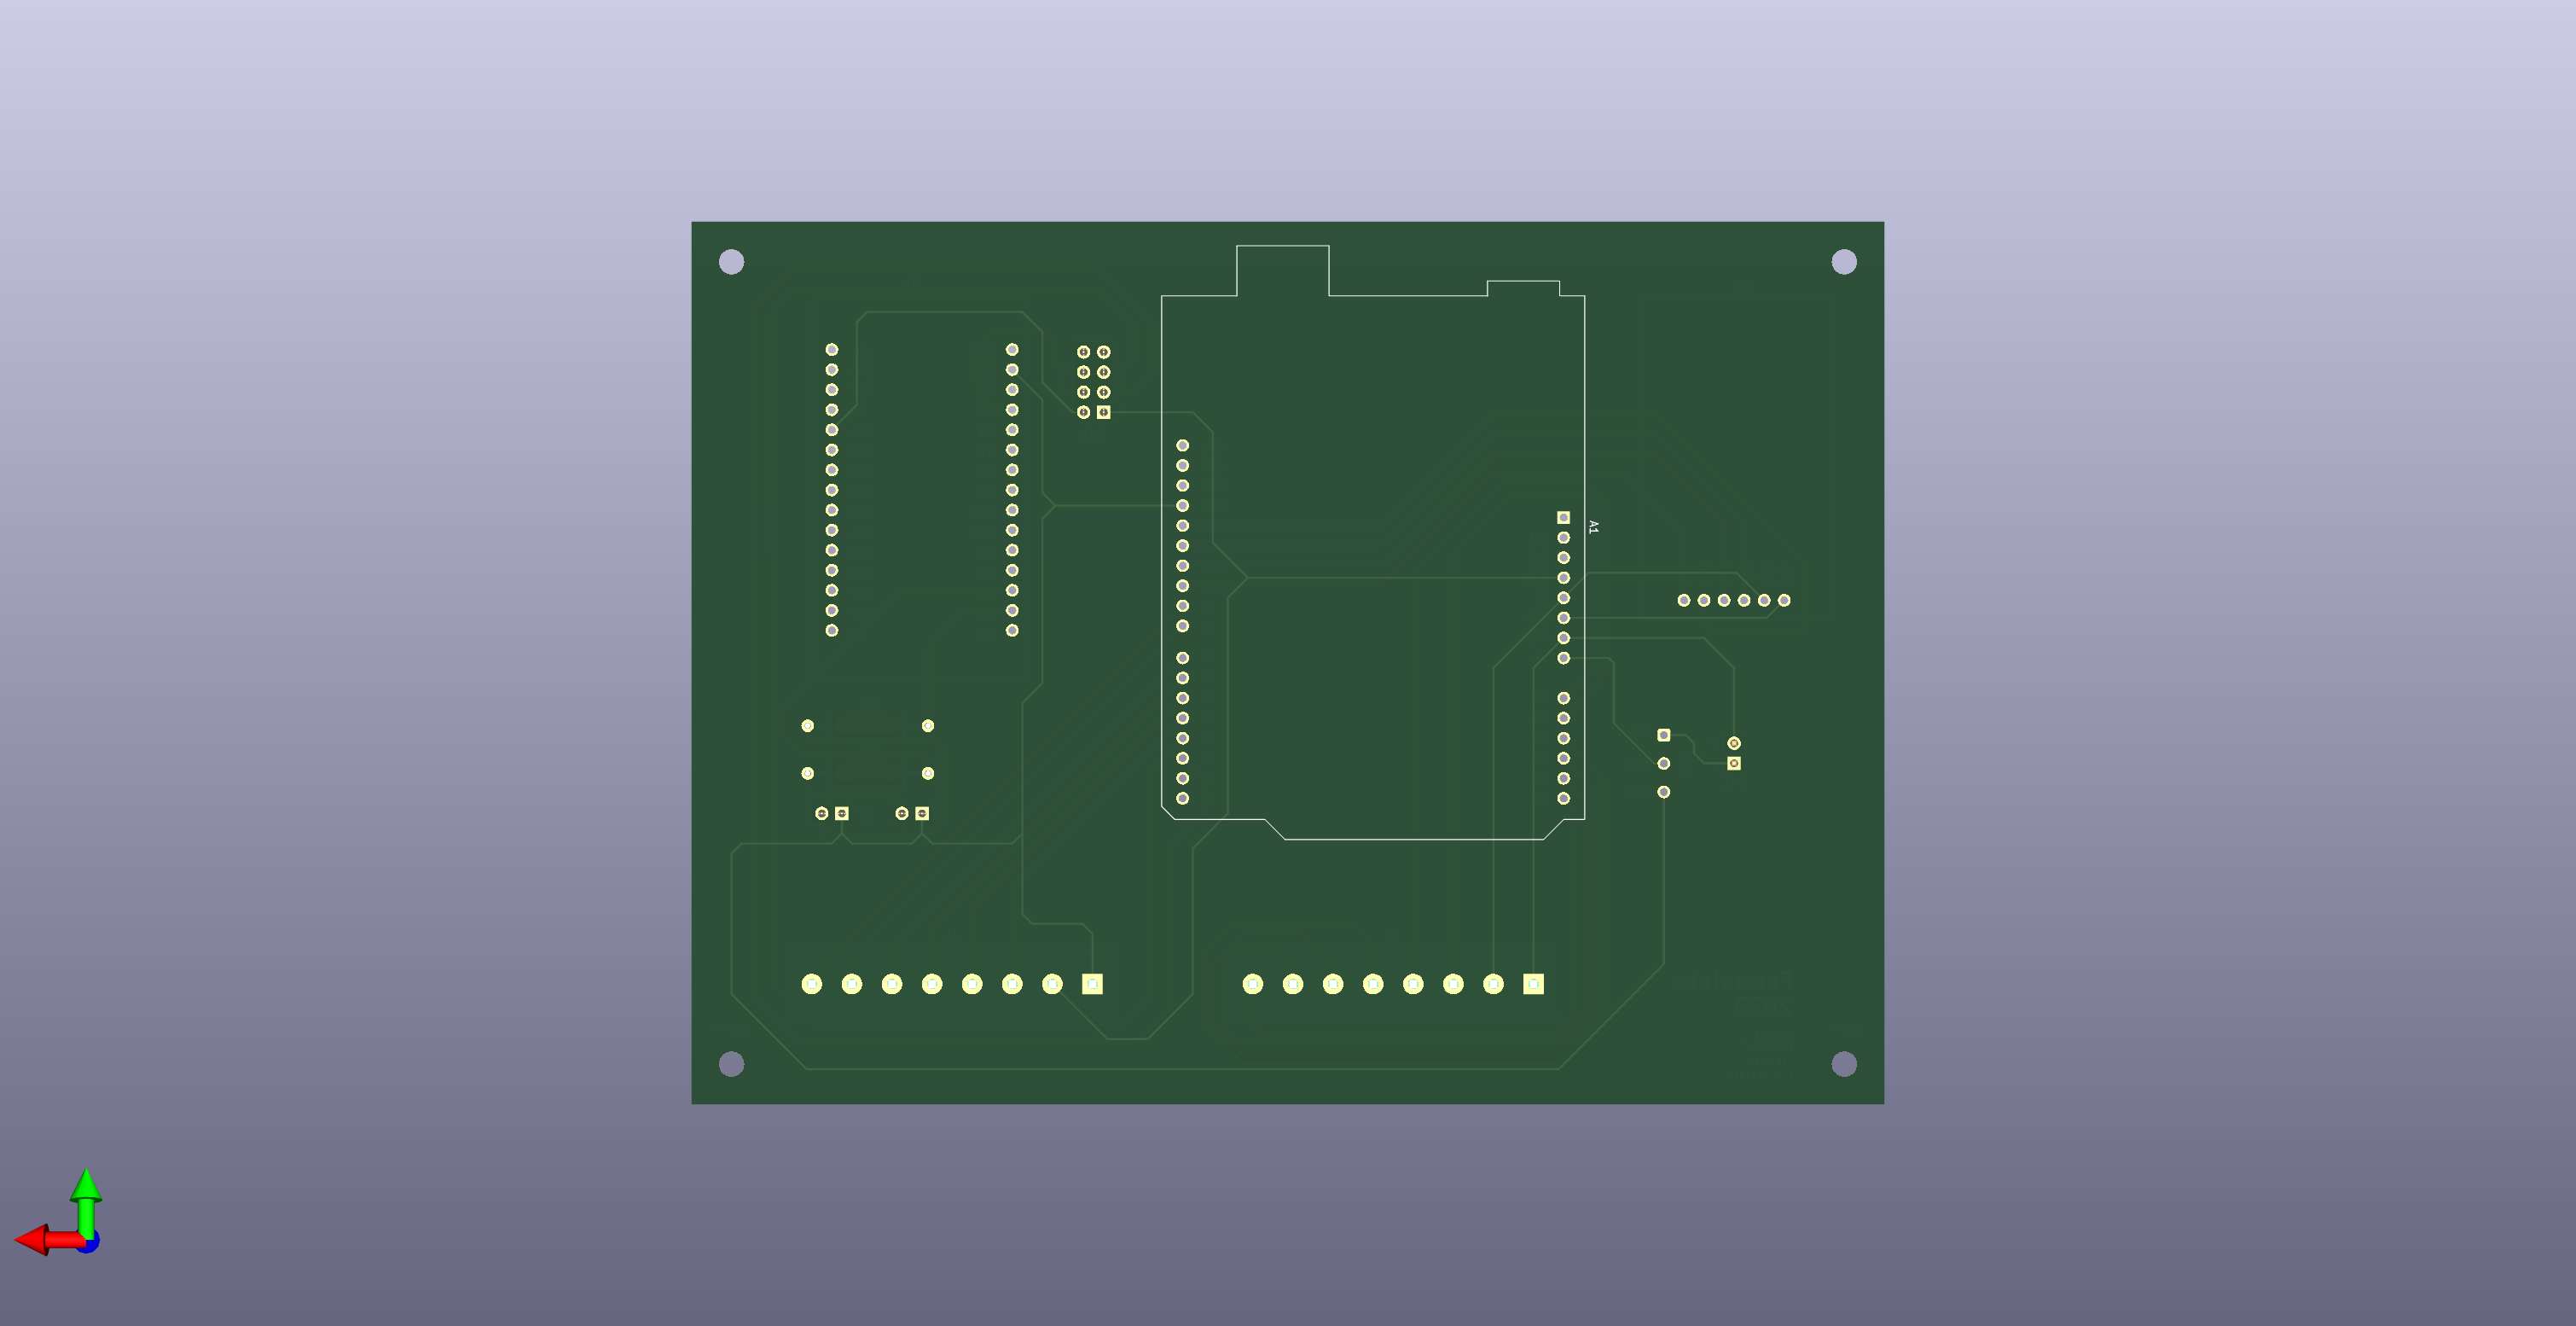
\includegraphics[width=1.1\textwidth]{PCB_Back_View}
  \caption{Bottom view of the PCB}
  \end{center}
  \end{figure}
  \newpage

\section{Communication Protocols}

\section{Reflection}

The information in this section will be used to evaluate the team members on the
graduate attribute of Problem Analysis and Design.  Please answer the following questions:

\begin{enumerate}
  \item What are the limitations of your solution?  Put another way, given
  unlimited resources, what could you do to make the project better? (LO\_ProbSolutions)

  Minimal PCB optimization was made to the layout. Primarily due to the time limitation of a lengthy and costly design, manufacture, test cycle for each PCB iteration, it was not feasible to optimize important PCB characteristics such as the absolute minimal layout size, noise minimization, and maximum structural rigidity. As a result, the team focused on achieving the functional solution in the shortest amount of time which limited optimization considerations. \\

  \item Give a brief overview of other design solutions you considered.  What
  are the benefits and tradeoffs of those other designs compared with the chosen
  design?  From all the potential options, why did you select documented design?
  (LO\_Explores)
\end{enumerate}
  A breadboard circuit with jumper cables and pin header connections was a simpler alternative solution to a PCB design. The breadboard circuit had some benefits such as the inexpensive monetary cost to design, manufacture, and test, and the short time to complete a complete circuit iteration. With that said however, the breadboard circuit lacked the ability to create robust wire connections between components and the ability to design a circuit with a smaller physical footprint. As a result, a PCB layout which functionally replaced the breadboard circuit was chosen as the ability to design a physically smaller circuit with rigid connections through soldered points and terminal blocks was possible. \\

\end{document}